% Ergebnisse und Analyse Diagramme.tex

\newcommand{\MergesortMaxArrayVerdoppelnMesswerte}{%
    \addplot[blue, mark=*] coordinates {
            (25000000,3017372600)
            (50000000,6315632400)
            (100000000,12777405700)
            (200000000,27203738300)
            (400000000,56441153000)
        };
    \addlegendentry{Mergesort Zufall}
}

\newcommand{\QuicksortMaxArrayVerdoppelnMesswerte}{%
    \addplot[green, mark=*] coordinates {
            (25000000,1528071600)
            (50000000,3248990900)
            (100000000,6653966800)
            (200000000,13778762100)
            (400000000,29074726600)
        };
    \addlegendentry{Quicksort Zufall}
}

\newcommand{\MergesortArrayVerdoppeln}{%
    \addplot[blue, mark=*] coordinates {
            (1,1000)
            (2,1300)
            (4,3100)
            (8,3200)
            (16,3500)
            (100,8700)
            (1000,97700)
            (2000,191700)
            (4000,354400)
            (8000,898800)
            (20000,1836000)
            (40000,3717200)
            (80000,7655300)
            (200000,19867700)
            (400000,40483400)
            (800000,83914700)
        };
    \addlegendentry{Mergesort}
}

\newcommand{\QuicksortArrayVerdoppeln}{%
    \addplot[green, mark=*] coordinates {
            (1,2700)
            (2,2800)
            (4,3100)
            (8,3800)
            (16,3300)
            (100,3000)
            (1000,34900)
            (2000,73100)
            (4000,148500)
            (8000,323600)
            (20000,826000)
            (40000,1777200)
            (80000,3888100)
            (200000,9835400)
            (400000,20598200)
            (800000,41432600)
        };
    \addlegendentry{Quicksort}
}

\newcommand{\QuicksortMaxArrayVerdoppelnMesswerteSortiert}{%
    \addplot[green!60!black, mark=*] coordinates {
            (25000000,165043900)
            (50000000,340924200)
            (100000000,726211400)
            (200000000,1550396900)
            (400000000,3130893200)
        };
    \addlegendentry{Quicksort Sortiert}
}

\newcommand{\MergesortgZufallG}{%
    \addplot[blue!, mark=*] coordinates {
            (1,1000)
            (2,1300)
            (4,3100)
            (8,3200)
            (10,4800)
            (16,3500)
            (100,8700)
            (1000,97700)
            (1200,115900)
            (2000,191700)
            (4000,354400)
            (8000,898800)
            (20000,1836000)
            (40000,3717200)
            (80000,7655300)
            (200000,19867700)
            (400000,40483400)
            (800000,83914700)
            (2000000,214959100)
            (4000000,441562800)
            (8000000,927314800)
            (25000000,3017372600)
            (40000000,5011540100)
            (50000000,6315632400)
            (100000000,12777405700)
            (200000000,27203738300)
            (400000000,56441153000)
        };
    \addlegendentry{Mergesort Zufall}
}

\newcommand{\QuicksortZufallG}{%
    \addplot[green, mark=*] coordinates {
            (1,2700)
            (2,2800)
            (4,3100)
            (8,3800)
            (10,400)
            (16,3300)
            (100,3000)
            (1000,34900)
            (1200,42900)
            (2000,73100)
            (4000,148500)
            (8000,323600)
            (20000,826000)
            (40000,1777200)
            (80000,3888100)
            (200000,9835400)
            (400000,20598200)
            (800000,41432600)
            (2000000,108526800)
            (4000000,218531900)
            (8000000,466862300)
            (25000000,1528071600)
            (40000000,2510531800)
            (50000000,3248990900)
            (100000000,6653966800)
            (200000000,13778762100)
            (400000000,29074726600)
        };
    \addlegendentry{Quicksort Zufall}
}

\newcommand{\MergesortgSortiertG}{%
    \addplot[blue!60!black, mark=*] coordinates {
            (1,200)
            (2,500)
            (4,1100)
            (8,1100)
            (10,900)
            (16,1600)
            (100,9100)
            (1000,63700)
            (1200,61900)
            (2000,109900)
            (4000,246500)
            (8000,502400)
            (20000,1676800)
            (40000,2321100)
            (80000,4356400)
            (200000,11443400)
            (400000,27704700)
            (800000,44349600)
            (2000000,119394700)
            (4000000,242919700)
            (8000000,504358000)
            (25000000,1609541400)
            (40000000,2733965500)
            (50000000,3314592200)
            (100000000,6854920900)
            (200000000,14495472700)
            (400000000,28117911500)
        };
    \addlegendentry{Mergesort Sortiert}
}

\newcommand{\QuicksortSortiertG}{%
    \addplot[green!70!black, mark=*] coordinates {
            (1,200)
            (2,300)
            (4,200)
            (8,200)
            (10,200)
            (16,300)
            (100,1000)
            (1000,4100)
            (1200,4800)
            (2000,8300)
            (4000,14800)
            (8000,34200)
            (20000,85300)
            (40000,179000)
            (80000,384300)
            (200000,1010200)
            (400000,2636000)
            (800000,4505800)
            (2000000,10849000)
            (4000000,22915200)
            (8000000,46914400)
            (25000000,165043900)
            (40000000,263361000)
            (50000000,340924200)
            (100000000,726211400)
            (200000000,1550396900)
            (400000000,3130893200)
        };
    \addlegendentry{Quicksort Sortiert}
}

\newcommand{\MergesortDupliziertG}{%
    \addplot[orange, mark=*] coordinates {
            (1,200)
            (2,500)
            (4,700)
            (8,1100)
            (10,1000)
            (16,1700)
            (100,8700)
            (1000,73500)
            (1200,90500)
            (2000,146000)
            (4000,298200)
            (8000,593500)
            (20000,1587000)
            (40000,3118300)
            (80000,6606800)
            (200000,15498400)
            (400000,31319100)
            (800000,64131400)
            (2000000,162417700)
            (4000000,328665200)
            (8000000,679938900)
            (25000000,2168311400)
            (40000000,3562459400)
            (50000000,4409952700)
            (100000000,8964155800)
            (200000000,18360003700)
            (400000000,38385447200)
        };
    \addlegendentry{Mergesort Dupliziert}
}

\newcommand{\QuicksortDupliziertG}{%
    \addplot[yellow, mark=*] coordinates {
            (1,100)
            (2,100)
            (4,200)
            (8,300)
            (10,300)
            (16,600)
            (100,3600)
            (1000,33300)
            (1200,31900)
            (2000,50000)
            (4000,98800)
            (8000,185300)
            (20000,599400)
            (40000,972900)
            (80000,1843800)
            (200000,5041800)
            (400000,9841900)
            (800000,19230300)
            (2000000,49799200)
            (4000000,102304100)
            (8000000,211552100)
            (25000000,666682700)
            (40000000,1061258600)
            (50000000,1314474600)
            (100000000,2723588000)
            (200000000,5627916700)
            (400000000,11116214800)
        };
    \addlegendentry{Quicksort Dupliziert}
}



\newcommand{\GrundlegendeLaufzeitenAbhaengigVonDerArraygroesseDiagrammA}{%
    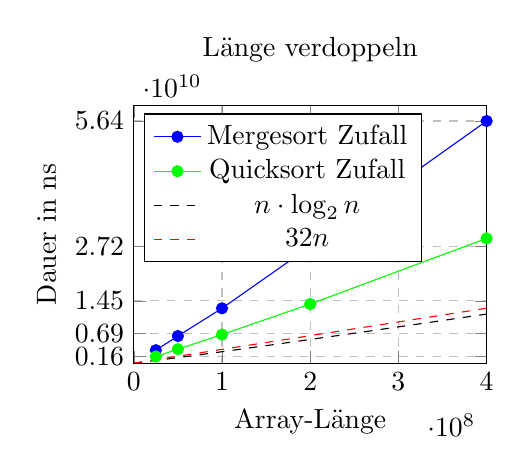
\begin{tikzpicture}
        \begin{axis}[
                title style={yshift=1.5ex},
                width=0.5\textwidth,
                height=0.4\textwidth,
                xlabel={Array-Länge},
                ylabel={Dauer in ns},
                title={Länge verdoppeln},
                xmin=0, xmax=4 * 10^8,
                ymin=0, ymax=6*10^10,
                grid=both,
                grid style=dashed,
                legend pos=north west,
                ytick={1609541400,6854920900,14495472700,27203738300,56441153000},
                % xtick={2^21,2^23,2^24,2^25},
                % xticklabels={$2^{21}$, $2^{23}$, $2^{24}$, $2^{25}$},
                % scaled x ticks=false,
                % scaled y ticks=false,
            ]
            \MergesortMaxArrayVerdoppelnMesswerte
            \QuicksortMaxArrayVerdoppelnMesswerte
            % n*log2(n)
            \addplot[black, dashed,domain=1:4e8, samples=100] {x*log2(x)};
            \addlegendentry{$n \cdot \log_2 n$}
            % n
            \addplot[red, dashed,domain=1:4e8, samples=100] {32*x};
            \addlegendentry{$32n$}
            % % log2(n)
            % \addplot[green, domain=1e7:4e8, samples=100] {log2(x)};
            % \addlegendentry{$\log_2 n$}
        \end{axis}
    \end{tikzpicture}%
}

\newcommand{\GrundlegendeLaufzeitenAbhaengigVonDerArraygroesseDiagrammB}{%
    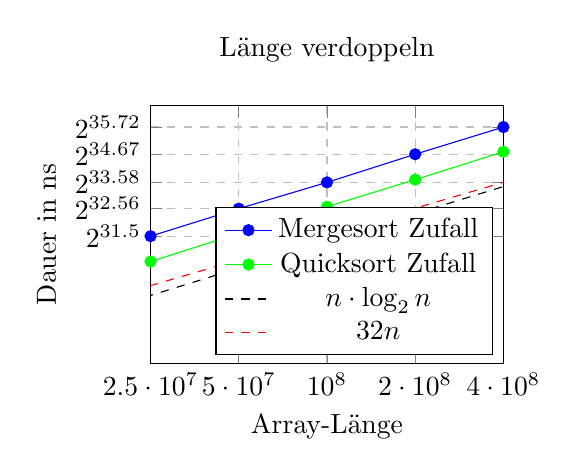
\begin{tikzpicture}
        \begin{axis}[
                title style={yshift=1.5ex},
                width=0.5\textwidth,
                height=0.4\textwidth,
                xlabel={Array-Länge},
                ylabel={Dauer in ns},
                title={Länge verdoppeln},
                xmin=2.5*10^7, xmax=4*10^8,
                ymin=10^8, ymax=1*10^11,
                grid=both,
                grid style=dashed,
                legend pos=south east,
                xmode=log,
                log basis x=10,
                xtick=data,
                xticklabels={$2.5\cdot10^7$, $5\cdot10^7$, $10^8$, $2\cdot10^8$, $4\cdot10^8$},
                ymode=log,
                log basis y=2,
                ytick=data,
                % xtick={2^21,2^23,2^24,2^25},
                % xticklabels={$2^{21}$, $2^{23}$, $2^{24}$, $2^{25}$},
                % scaled x ticks=false,
                % scaled y ticks=false,
            ]
            \MergesortMaxArrayVerdoppelnMesswerte
            \QuicksortMaxArrayVerdoppelnMesswerte
            % n*log2(n)
            \addplot[black, dashed,domain=1e7:4e8, samples=100] {x*log2(x)};
            \addlegendentry{$n \cdot \log_2 n$}
            % n
            \addplot[red, dashed,domain=1:4e8, samples=100] {32*x};
            \addlegendentry{$32n$}
            % % 64*x - 1000000000
            % \addplot[gray, dashed,domain=2*10^7:4e8, samples=100] {64*x - 10^9};
            % \addlegendentry{$64 \cdot n - 10^9$}
        \end{axis}
    \end{tikzpicture}%
}

\newcommand{\GrundlegendeLaufzeitenAbhaengigVonDerArraygroesseDiagrammC}{%
    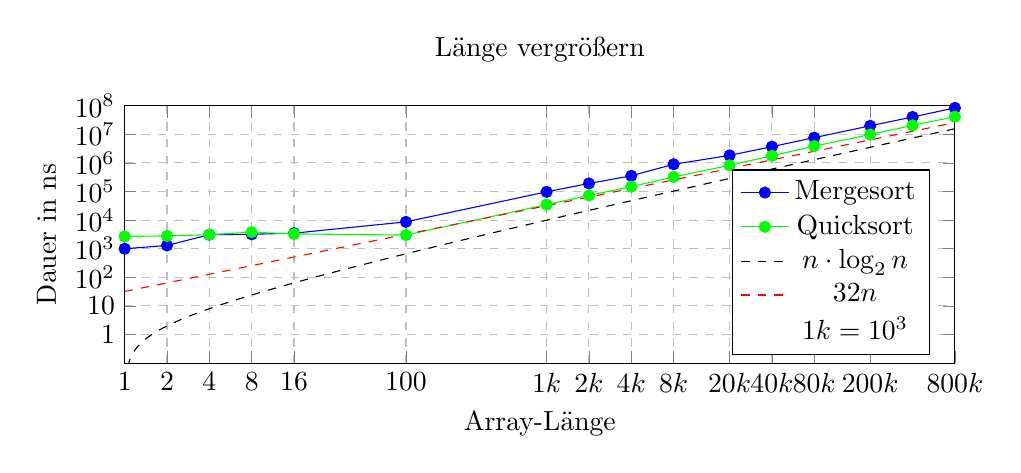
\begin{tikzpicture}
        \begin{axis}[
                title style={yshift=1.5ex},
                width=1\textwidth,
                height=0.4\textwidth,
                xlabel={Array-Länge},
                ylabel={Dauer in ns},
                title={Länge vergrößern},
                xmin=1, xmax=800000,
                ymin=0.1, ymax=1*10^8,
                grid=both,
                grid style=dashed,
                legend pos=south east,
                xmode=log,
                log basis x=10,
                %xtick=data,
                xtick={1,2,4,8,16,100,1000,2000,4000,8000,20000,40000,80000,200000,800000},
                xticklabels={
                        $1$,$2$,$4$,$8$,$16$,
                        $100$,$1k$,
                        $2k$,$4k$,$8k$,
                        $20k$,$40k$,$80k$,
                        $200k$,$800k$
                    },
                ymode=log,
                log basis y=10,
                ytick={1,10,10^2,10^3,10^4,10^5,10^6,10^7,10^8},
                yticklabels={$1$,$10$,$10^{2}$,$10^{3}$,$10^{4}$,$10^{5}$,$10^{6}$,$10^{7}$,$10^{8}$},
                % scaled x ticks=false,
                % scaled y ticks=false,
            ]
            \MergesortArrayVerdoppeln
            \QuicksortArrayVerdoppeln
            % n*log2(n)
            \addplot[black, dashed,domain=1:800000, samples=1000] {x*log2(x)};
            \addlegendentry{$n \cdot \log_2 n$}
            % n
            \addplot[red, dashed,domain=1:800000, samples=100] {32*x};
            \addlegendentry{$32n$}
            \addlegendimage{empty legend}
            \addlegendentry{$1k = 10^3$}
        \end{axis}
    \end{tikzpicture}%
}

\newcommand{\EinflussDesListentypsDiagrammA}{%
    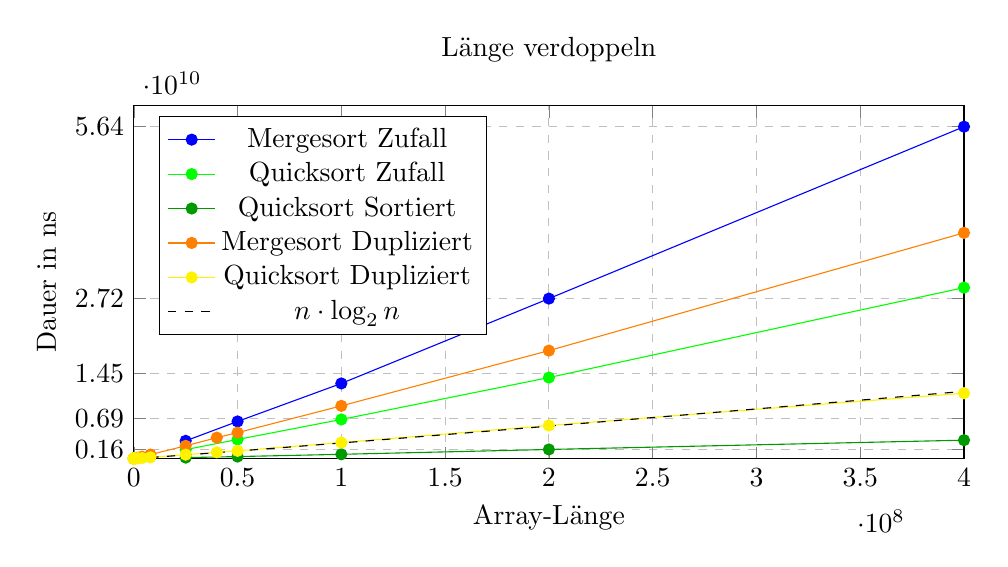
\begin{tikzpicture}
        \begin{axis}[
                title style={yshift=1.5ex},
                width=1\textwidth,
                height=0.5\textwidth,
                xlabel={Array-Länge},
                ylabel={Dauer in ns},
                title={Länge verdoppeln},
                xmin=0, xmax=4 * 10^8,
                ymin=0, ymax=6*10^10,
                grid=both,
                grid style=dashed,
                legend pos=north west,
                ytick={1609541400,6854920900,14495472700,27203738300,56441153000},
                % xtick={2^21,2^23,2^24,2^25},
                % xticklabels={$2^{21}$, $2^{23}$, $2^{24}$, $2^{25}$},
                % scaled x ticks=false,
                % scaled y ticks=false,
            ]
            \MergesortMaxArrayVerdoppelnMesswerte
            \QuicksortMaxArrayVerdoppelnMesswerte
            \QuicksortMaxArrayVerdoppelnMesswerteSortiert
            \MergesortDupliziertG
            \QuicksortDupliziertG
            % n*log2(n)
            \addplot[black, dashed,domain=1:4e8, samples=100] {x*log2(x)};
            \addlegendentry{$n \cdot \log_2 n$}
        \end{axis}
    \end{tikzpicture}%
}

\newcommand{\EinflussDesListentypsDiagrammB}{%
    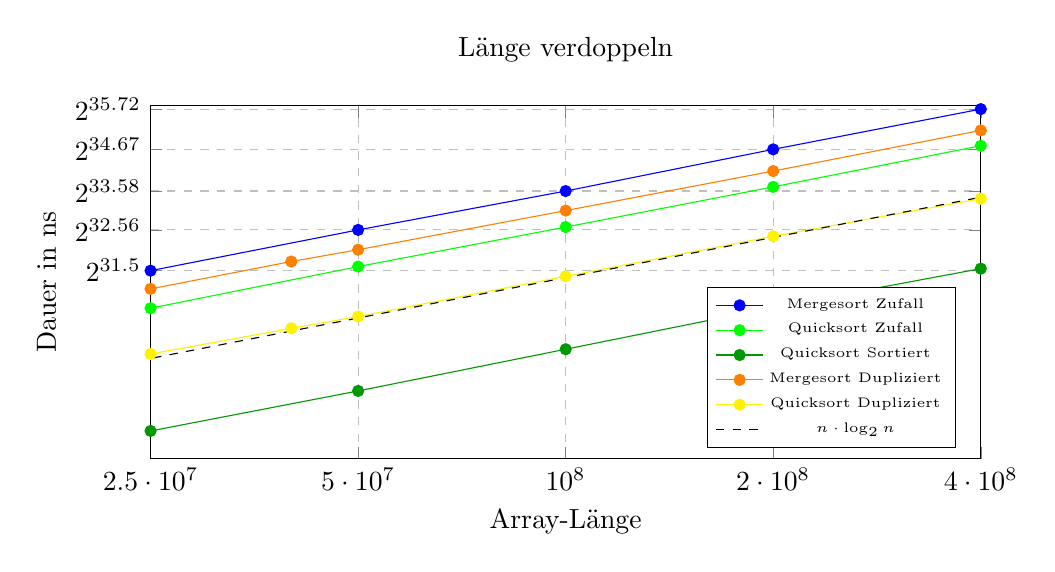
\begin{tikzpicture}
        \begin{axis}[
                title style={yshift=1.5ex},
                width=1\textwidth,
                height=0.5\textwidth,
                xlabel={Array-Länge},
                ylabel={Dauer in ns},
                title={Länge verdoppeln},
                xmin=2.5*10^7, xmax=4*10^8,
                ymin=10^8, ymax=6*10^10,
                grid=both,
                grid style=dashed,
                legend pos=south east,
                legend style={font=\tiny},
                xmode=log,
                log basis x=10,
                xtick=data,
                xticklabels={$2.5\cdot10^7$, $5\cdot10^7$, $10^8$, $2\cdot10^8$, $4\cdot10^8$},
                ymode=log,
                log basis y=2,
                ytick=data,
                % xtick={2^21,2^23,2^24,2^25},
                % xticklabels={$2^{21}$, $2^{23}$, $2^{24}$, $2^{25}$},
                % scaled x ticks=false,
                % scaled y ticks=false,
            ]
            \MergesortMaxArrayVerdoppelnMesswerte
            \QuicksortMaxArrayVerdoppelnMesswerte
            \QuicksortMaxArrayVerdoppelnMesswerteSortiert
            \MergesortDupliziertG
            \QuicksortDupliziertG
            % n*log2(n)
            \addplot[black, dashed,domain=1e7:4e8, samples=100] {x*log2(x)};
            \addlegendentry{$n \cdot \log_2 n$}
        \end{axis}
    \end{tikzpicture}%
}

\newcommand{\EinflussDesListentypsDiagrammC}{%
    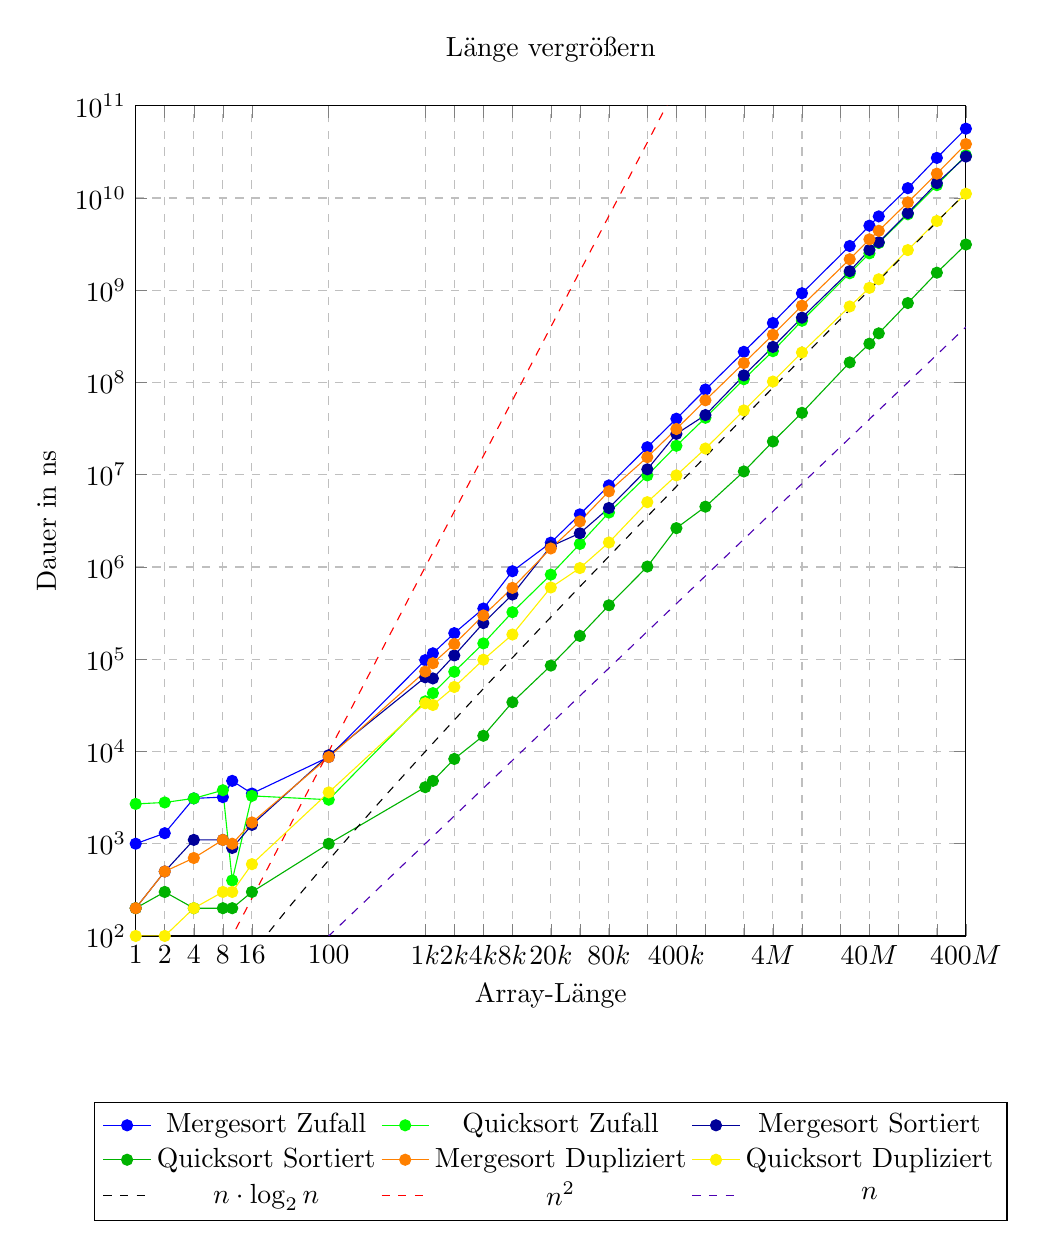
\begin{tikzpicture}
        \begin{axis}[
                title style={yshift=1.5ex},
                width=1\textwidth,
                height=1\textwidth,
                xlabel={Array-Länge},
                ylabel={Dauer in ns},
                title={Länge vergrößern},
                xmin=1, xmax=400000000,
                ymin=100, ymax=1*10^11,
                grid=both,
                grid style=dashed,
                % legend pos=south east,
                legend style={
                        at={(0.5,-0.2)},
                        anchor=north,
                        legend columns=3
                    },
                xmode=log,
                log basis x=10,
                %xtick=data,
                xtick={1,2,4,8,16,100,1000,2000,4000,8000,20000,40000,80000,200000,400000,800000,2000000,4000000,8000000,20000000,40000000,80000000,200000000,400000000},
                xticklabels={
                        $1$,$2$,$4$,$8$,$16$,
                        $100$,$1k$,
                        $2k$,$4k$,$8k$,
                        $20k$,$$,$80k$,
                            $ $,$400k$,$ $,
                            $ $,$4M$,$$,
                        $$,$40M$,$$,
                        $$,$400M$,$$
                    },
                ymode=log,
                log basis y=10,
                ytick={1,10,10^2,10^3,10^4,10^5,10^6,10^7,10^8,10^9,10^10,10^11},
                yticklabels={$1$,$10$,$10^{2}$,$10^{3}$,$10^{4}$,$10^{5}$,$10^{6}$,$10^{7}$,$10^{8}$,$10^{9}$,$10^{10}$,$10^{11}$}
                % scaled x ticks=false,
                % scaled y ticks=false,
            ]
            \MergesortgZufallG
            \QuicksortZufallG
            \MergesortgSortiertG
            \QuicksortSortiertG
            \MergesortDupliziertG
            \QuicksortDupliziertG
            % n*log2(n)
            \addplot[black, dashed,domain=1:400000000, samples=1000] {x*log2(x)};
            \addlegendentry{$n \cdot \log_2 n$}
            % n^2
            \addplot[red, dashed,domain=1:4e8, samples=100] {x*x};
            \addlegendentry{$n^2$}
            % n
            \addplot[blue!70!red, dashed,domain=1:4e8, samples=100] {x};
            \addlegendentry{$n$}
        \end{axis}
    \end{tikzpicture}%
}